\section{Preliminary results}
\label{sec:prelim}
The evaluation is in progress. Results so far are mixed. The full
methodology and numbers are in the working
notes\footnote{K.~Wiechecki, \emph{Dictionary learning as unsupervised
steering-vector generation: Ontologizers vs.\ sparse autoencoders on
SONAR sentence embeddings}, working notes, in preparation; distributed
with this proposal.}; the headlines are summarized here. Two models
recur throughout and are named once now. The notes' reference model,
\texttt{resid\_nc} (372{,}600 steps), is the model behind the notes'
tables, including Tables~\ref{tab:prelim-pareto}
and~\ref{tab:prelim-headcoh}. Its sibling \texttt{resid\_nc\_hm} is
the same configuration plus the batch mean-entropy bonus the notes
propose as the freeze fix, trained to 4.38M steps; the new experiments
reported here use its final checkpoint unless stated otherwise.

The notes carry one caveat about the reference: ``layer 4 froze 22/32
heads late in temperature annealing and is mildly harmful.'' A
diagnostic over both training histories (frozen: top classification
share ${\geq}0.95$ and churn ${\leq}0.02$) bears the caveat out and
locates the fix (Figure~\ref{fig:freeze}). In \texttt{resid\_nc}, the
top layer (layer 4 of 0--4) begins freezing near step 190k, well after
the anneal, reaches 27 of 32 by step 210k and 28 at its peak, and is
still frozen at the last checkpoint; the count differs from the notes'
22 under this criterion, the layer and the persistence do not. In
\texttt{resid\_nc\_hm} the late freeze never occurs: what remains is
an early annealing transient (22 of 32 at layer 1 of 0--4 at step 10k,
with 16, 11, and 4 of 32 at layers 2, 3, and 0) that recovers
completely by step 30k, leaving the final checkpoint unfrozen
everywhere. The mean-entropy bonus does what the notes proposed it
for.

\begin{figure}[tp]\centering
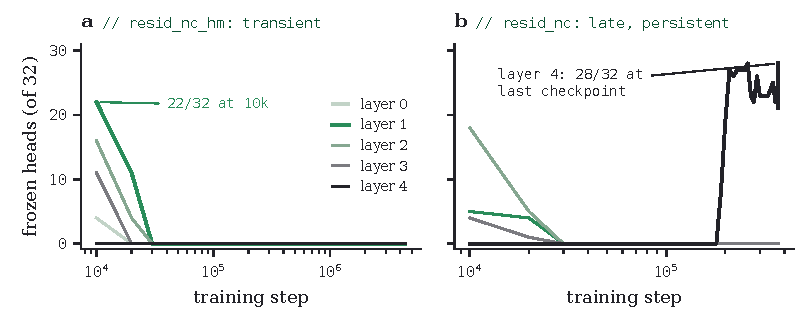
\includegraphics[width=\linewidth]{figures/fig-freeze.pdf}
\caption{Frozen heads per layer over training (frozen: top
classification share ${\geq}0.95$, churn ${\leq}0.02$). Left:
\texttt{resid\_nc\_hm}, with the mean-entropy bonus, has only an early
annealing transient, peaking at 22/32 in layer 1 at step 10k and
recovering to zero everywhere by step 30k. Right: \texttt{resid\_nc},
the notes' reference, carries the caveat: a post-anneal layer-4 freeze
from ${\sim}$190k that persists through its last checkpoint.}
\label{fig:freeze}
\end{figure}

Four retrains of the \texttt{resid\_nc\_hm} configuration, a
zero-change control and three single-knob variants (372k steps each),
close the question of what drives the remaining transient. The control
reproduces it head-for-head (22/32 at layer 1 at step 10k, zero
everywhere by 30k) and shows no late freeze over its horizon.
Stretching the temperature anneal from 50k to 150k steps attenuates
and spreads the transient (peak 14/32 at layer 1 at step 30k, clear by
50k); raising winner dropout from $0.1$ to $0.25$ tracks the control
to within two heads at the peak, and holding the classification-noise
floor at its starting value changes nothing at all
(Figure~\ref{fig:variants}). The transient belongs to the temperature
schedule alone, and every retrain ends unfrozen everywhere.

\begin{figure}[tp]\centering
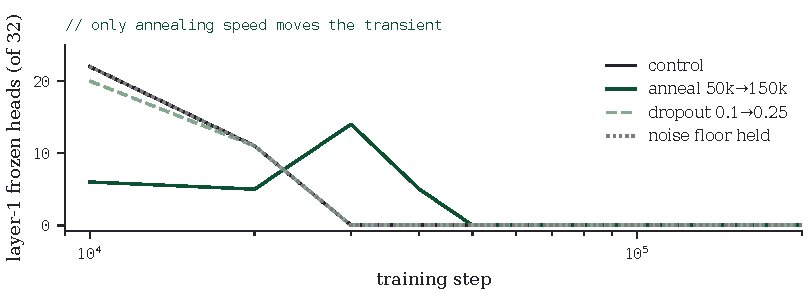
\includegraphics[width=\linewidth]{figures/fig-variants.pdf}
\caption{The early transient under the four retrains, layer-1 frozen
count. The noise-floor variant overlaps the control exactly and the
dropout variant tracks it to within two heads at the peak; only
stretching the temperature anneal moves the curve, trading peak height
for duration.}
\label{fig:variants}
\end{figure}

\subsection{Reconstruction quality}
Contrast-set structure is expensive. The plain-SAE frontier dominates
the Ontologizer's deviation code at every capacity tested
(Table~\ref{tab:prelim-pareto}), and the grouped-simplex constraint
alone costs roughly $40\times$ in weighted fraction of variance
unexplained. Here $\mathrm{FVU}_w$ is whitened MSE over the whitened
variance of a constant predictor, and the deviation code is a per-head
top-$m$ truncation around the measured mean classification
$\mathbb{E}[p]$. The train/eval asymmetry carries over from the notes: the
Ontologizer trained on the full cache including the evaluation tail,
while the SAEs excluded it; a fresh-encoded evaluation set is blocked
on a data source (Section~\ref{sec:future-completing}).

\begin{table}[tp]\centering\small
\begin{tabular}{@{}lrrr@{}}
\toprule
point & coeffs & index bits & $\mathrm{FVU}_w$ \\
\midrule
onto $m{=}0$ ($\mathbb{E}[p]$ origin) & 0 & 0 & 1.001 \\
onto hard (argmax)                  & 0 & 800 & 17.34 \\
sae k32 tier ($m{=}5120/11264$, incl.\ p5, s43) & 32 & $\sim$400 & 0.494--0.509 \\
sae k32 bilinear                    & 32 & 394 & 0.602 \\
onto dev $m{=}1$                    & 160 & 800 & 0.677 \\
sae g160top1                        & 160 & 1972 & 0.274 \\
sae k160 ($m{=}11264$)              & 160 & 2154 & 0.258 \\
onto dev $m{=}2$                    & 320 & 1600 & 0.497 \\
onto dev $m{=}4$                    & 640 & 3200 & 0.289 \\
onto dev $m{=}8$                    & 1280 & 6400 & 0.094 \\
sae k5120 ($m{=}11264$, $L_0{\approx}1520$) & 1520 & 20455 & \textbf{0.00011} \\
onto dev $m{=}16$                   & 2560 & 12800 & 0.0082 \\
sae g160softmax                     & 5120 & 0 & \textbf{0.00436} \\
onto soft ($m{=}32$)                & 5120 & 0 & 0.00538 \\
\bottomrule
\end{tabular}
\caption{Reconstruction against code capacity on the shared evaluation
tail, reproduced from the working notes. Ontologizer points are
top-$m$ deviation truncations around the measured $\mathbb{E}[p]$
origin; SAE points use measured eval $L_0$. The plain-SAE frontier
dominates the Ontologizer's deviation code at every measured capacity;
the gap is the price of contrast-set structure.}
\label{tab:prelim-pareto}
\end{table}

\subsection{Orthogonality}
\label{sec:prelim-orth}
Trained heads carry the signature the steering goal predicts: within-head
decode directions repel, with 96\% of Ontologizer heads below a
random-group null (Table~\ref{tab:prelim-headcoh}). Heads form
well-separated contrast sets rather than semantic clusters, in both the
Ontologizer and its single-layer grouped-softmax analogue.
This is the within-head axis: it says the $k$ entries of a head spread
apart, not that distinct heads occupy disjoint coordinates. The
between-head disjoint support of Section~\ref{sec:disjoint} is a
separate claim and is not tested here.

\begin{table}[tp]\centering\small
\begin{tabular}{@{}lrrrr@{}}
\toprule
grouping & groups & mean $z_{\cos}$ & frac $z{>}2$ & frac $z{<}{-}2$ \\
\midrule
g160top1 (trained, hard)      & 160 & $+161.3$ & 1.00 & 0.00 \\
k32 discovered (\texttt{m11264}) & 359 & $+1.7$ & 0.36 & 0.02 \\
onto heads (trained, soft)    & 160 & $-17.6$ & 0.04 & \textbf{0.96} \\
g160softmax (trained, soft)   & 160 & $-14.7$ & 0.00 & \textbf{1.00} \\
\bottomrule
\end{tabular}
\caption{Within-head decode-direction coherence, $z$-scored against
size-matched same-pool nulls ($n_{\text{null}}{=}500$), reproduced from
the working notes. Softmax-trained heads are anti-coherent: in
96--100\% of heads the entries' decode directions repel, so heads hold
well-separated contrastive alternatives rather than semantic clusters.
Hard per-group selection shows the opposite signature.}
\label{tab:prelim-headcoh}
\end{table}

\subsection{Categorical structure}
Categorical form, exhaustive and exclusive, exists precisely when it is
trained in as hard selection. It never emerges spontaneously, and it is
not recoverable post hoc.

\subsection{Automated interpretability}
\label{sec:prelim-autointerp}
Per-latent evaluation lenses systematically mis-measure classifier
codes, whose content lives in partitions rather than latent magnitudes.
Blinded describability tracks code density rather than architecture,
and parameter-space decodes of feature directions fail as descriptions
outright.

A head-level pass over \texttt{resid\_nc} (step 372{,}600) tests this
directly; its frozen top layer is a caveat for any layer-4 heads in
the sample. Decoding descriptions from dictionary parameters fails at
the partition level as it does per latent (median self accuracy
$0.02$).
Activation-grounded head descriptions do no better than a null pairing
at the current sample size ($n{=}20$ heads per condition, median
accuracy $0.083$ against $0.125$), and a head's detection accuracy is
uncorrelated with the mean describability of its latents (Spearman
$+0.07$ over 30 head--lens pairs, 15 heads under each lens; neither
per-lens value distinguishable from zero). The two lenses disagree and
neither shows above-chance head-level signal, so the mis-measurement
argument predicts an advantage the current sample fails to deliver.

\subsection{Steering fidelity}
There is a causally verified existence proof: forcing a single
classification in the first layer reliably steers decodes into Burmese
while otherwise preserving content. Joint interventions compose
approximately additively (median cosine between summed and joint decode
deltas at least $0.95$, exact in the final layer). Text fidelity for
soft codes sits near the likelihood ceiling, while the sparse SAE tier
starts at roughly $0.75$ collateral, so low-collateral steering is
currently exclusive to the soft architectures.

The matched-budget overlay against supervised baselines is now in
(Table~\ref{tab:steer-overlay}): difference-of-means, linear-probe, and
forced-classification arms with a random-direction floor, medians over
24 language--magnitude cells per arm on language steering. Each arm
wins its own effect frame, as expected. On the shared
difference-of-means frame, classification forcing moves decodes along
the target direction $0.43\times$ as far as supervised steering does,
and lands well ahead of probe directions. The collateral column is the
check on all of it: every arm's collateral, supervised steering
included, sits at the random-direction floor ($0.72$--$0.78$), and none
materially beats it. On task naturalness the arms are so far
indistinguishable (Figure~\ref{fig:naturalness}): chrF against
unsteered decodes falls from ${\sim}0.35$ at magnitude $0.25$ to
${\sim}0.15$ at magnitude $1.0$ for the difference-of-means and
forced-classification arms, with probe and random decaying in parallel
from ${\sim}0.38$ to ${\sim}0.20$, and forced classifications tracking
difference-of-means within noise throughout. A blinded human-rating
sheet (120 items) is prepared but unscored.

\begin{table}[tp]\centering\small
\begin{tabular}{@{}lrrrr@{}}
\toprule
arm & eff (native) & eff (dm frame) & hit rate & collateral \\
\midrule
difference of means    & 0.337 & 0.337 & 0.250 & 0.757 \\
classification forcing & 0.394 & 0.146 & 0.125 & 0.778 \\
linear probe           & 0.293 & 0.028 & 0.000 & 0.720 \\
random direction       & --    & --    & --   & 0.721 \\
\bottomrule
\end{tabular}
\caption{Language steering under matched intervention budgets on
\texttt{resid\_nc\_hm}'s final checkpoint; medians over 24
language--magnitude cells per arm.
Effect is displacement along the arm's own direction (native) and along
the shared difference-of-means direction (dm frame); hit rate is the
fraction of steered decodes reaching the median projection of genuine
target-language rows on the shared frame; collateral is content change
on unrelated dimensions, with the random-direction row as the floor. Each arm dominates its native frame; on the shared frame
classification forcing reaches $0.43\times$ the supervised effect.
Every arm's collateral sits at the random floor at these budgets.}
\label{tab:steer-overlay}
\end{table}

\begin{figure}[tp]\centering
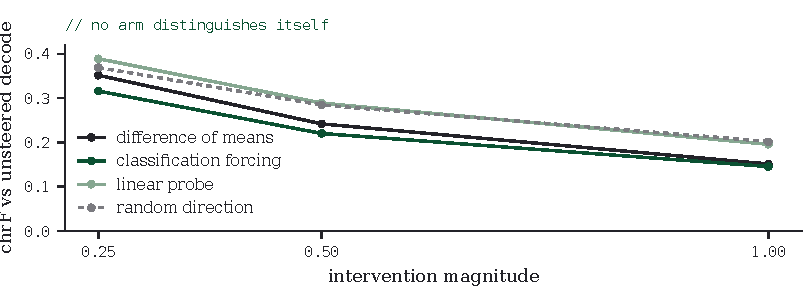
\includegraphics[width=\linewidth]{figures/fig-naturalness.pdf}
\caption{chrF between steered and unsteered decodes by intervention
magnitude. All four arms, the random direction included, damage the
decode at nearly the same rate; no arm buys naturalness at matched
magnitude.}
\label{fig:naturalness}
\end{figure}

The decisive comparison, though, is architectural. A single-layer grouped-softmax
SAE reproduces the Ontologizer's code structure, contrastive signature,
and text fidelity at better reconstruction with half the parameters. It
is the rival null hypothesis the full architecture must beat on
steering quality and task naturalness, and that comparison is where the
work currently sits.

\subsection{Seed stability}
\label{sec:prelim-seed}
Partitions do not reproduce across seeds at matched training. A second
run of the \texttt{resid\_nc\_hm} configuration from a different seed,
compared at matched training (370k steps on both sides), matches
essentially nothing
(Figure~\ref{fig:seed}): no head pair and at most $0.3\%$ of entries
clear a $0.3$ cosine threshold on dictionary geometry, and
activation-frame containment over a shared evaluation batch is at most
$0.001$ at any threshold, against $0.31$/$0.24$/$0.15$/$0.03$ for the
k32 SAE and its own seed replica across the four match thresholds
($0.3$--$0.9$). The metric itself has headroom: the same run compared
against itself $2{,}600$ steps apart scores $1.000$ on geometry at
every threshold, and $0.65$ at the loosest activation threshold
(falling to $0.20$ at the strictest), so the activation frame has a
self-ceiling well below one and the cross-seed numbers sit far below
both ceilings. At matched training the Ontologizer's partitions are
less reproducible across seeds than the SAE latents this proposal
criticizes. A replica carried to \texttt{resid\_nc\_hm}'s full $4.4$M
steps is the remaining control.

\begin{figure}[tp]\centering
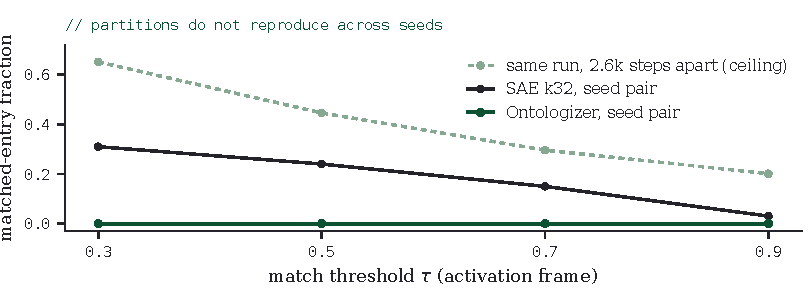
\includegraphics[width=\linewidth]{figures/fig-seed.pdf}
\caption{Cross-seed matched-entry fraction on the activation frame by
threshold. The same-run pair bounds what the metric can detect ($0.65$
at $\tau{=}0.3$); the k32 SAE pair reproduces partially; Ontologizer
partitions reproduce not at all.}
\label{fig:seed}
\end{figure}

\subsection{Development over training}
\label{sec:prelim-devinterp}
Tracking \texttt{resid\_nc\_hm}'s full 448-checkpoint history gives
the devinterp question a first answer. The tracked statistic applies
Table~\ref{tab:prelim-headcoh}'s $z$-score machinery to the refit
end-to-end direction matrix rather than to raw dictionary decode
directions, so the two are not directly comparable: the notes' raw
decode directions repel ($z{=}{-}17.6$, measured on \texttt{resid\_nc}
at 372.6k steps) while the refit directions on
\texttt{resid\_nc\_hm}'s final checkpoint cohere ($z{=}{+}72$); the
statistics differ in both instrument and substrate, and the refit
frame folds in the shared decoder and cross-layer interactions. On that statistic the
shape is rise, peak, and partial relaxation
(Figure~\ref{fig:devinterp}): mean within-head $z_{\cos}$ climbs from
$1.8$ at step 10k to a peak of $119$ near step 370k (median $123$,
every head above $z{=}2$), then relaxes over the remaining $4$M steps
to $72$ at the final checkpoint (median $105$, $0.79$ above $z{=}2$).
The code itself moves the other way after the annealing transient:
per-sample entropy returns to $4.5$ bits of a $5$-bit maximum and usage
KL falls toward uniform: relative to initialization the consolidation
is in the geometry the classifications write, while the classifications
themselves stay soft.

\begin{figure}[tp]\centering
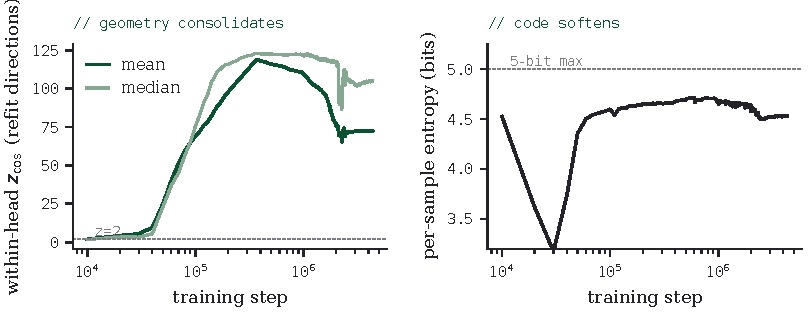
\includegraphics[width=\linewidth]{figures/fig-devinterp.pdf}
\caption{The 448-checkpoint training history. Left: within-head
coherence of refit end-to-end directions, $z$-scored against
size-matched nulls; rise, peak near step 370k, partial relaxation.
Right: mean per-sample classification entropy returns toward the
$5$-bit maximum after the annealing transient. Geometry consolidates
while the code itself stays soft.}
\label{fig:devinterp}
\end{figure}

\subsection{HSIC-bottleneck ablation}
\label{sec:prelim-hsic}
An HSIC bottleneck is a candidate replacement for the auxiliary
losses: maximize dependence with the reconstruction target while
penalizing dependence between heads. Both arms are in, retrained on
the \texttt{resid\_nc\_hm} configuration to 372k steps. Replacing the
four auxiliary terms with the HSIC objective destroys head health: a
late, persistent freeze takes 77 of 160 heads by the final checkpoint,
one layer entirely (layer 3, 32/32 from step 80k), while
reconstruction lands slightly behind the control (tail-mean training
MSE $3.7{\times}10^{-5}$ against $3.4{\times}10^{-5}$). Adding HSIC on
top of the auxiliary terms is worse on both counts: reconstruction
$4.4{\times}10^{-5}$, and 41 of 160 heads still frozen at the end,
layer 3 fully frozen by 80k with only partial thaw
(Figure~\ref{fig:hsic}). The failure mode is \texttt{resid\_nc}'s late
freeze, not the transient, which places the bottleneck and the
mean-entropy bonus in direct opposition: the bonus prevents exactly
what HSIC induces. As formulated the bottleneck is not a replacement,
and it is not an addition either.

\begin{figure}[tp]\centering
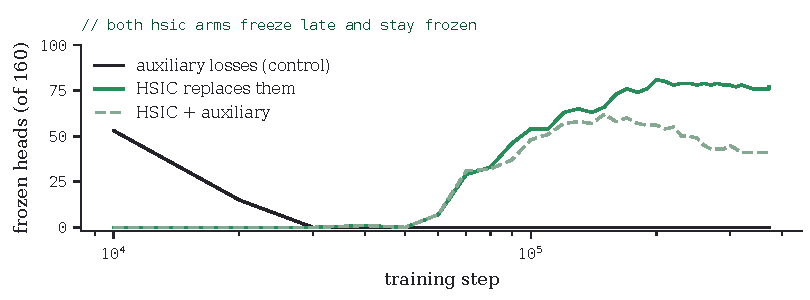
\includegraphics[width=\linewidth]{figures/fig-hsic.pdf}
\caption{Total frozen heads over training for the three loss
configurations, all on the \texttt{resid\_nc\_hm} configuration at
372k steps. The auxiliary-loss control's freeze is the early transient
and resolves; both HSIC arms develop the late, persistent freeze
instead, and the auxiliary terms only partially thaw it.}
\label{fig:hsic}
\end{figure}

\subsection{Against the desiderata}
Scored against the introduction: causal is currently positive (the
forced-classification steering result is causally verified), composable
is positive (interventions compose approximately additively), and
closed-form is negative (parameter-space decodes fail as descriptions).
Seed stability is measured on both sides: the k32 SAE pair matches at
$0.31$ down to $0.03$ as the threshold tightens while Ontologizer
partitions match at zero (Section~\ref{sec:prelim-seed}). The residual
stack's one quantified credit remains roughly $3\times$ adaptive
compensation under truncation (the shrinkage decomposition in the
working notes). Of the outstanding comparisons, the
steering overlay is a qualified positive, task naturalness is so far a
wash, and seed stability is a clear negative; the reconstruction price
Table~\ref{tab:prelim-pareto} puts on the architecture stands.


